\pagestyle{empty}

\definecolor{plop}{HTML}{4D7186}
\begin{textblock}{1}(0,0)
    \noindent\textcolor{white}{\rule{\paperwidth}{.55\paperheight}}
\end{textblock}


\begin{textblock}{1}(0,.55)
    \noindent\textcolor{gray}{\rule{\paperwidth}{.45\paperheight}}
\end{textblock}
\begin{figure}[ht]
   \centering  
   
\includegraphics[width=1.0\textwidth]{CSE.png} 
\end{figure}  
%\begin{textblock}{.3}(.3,.05)
%    \begin{center}
%        \centering 
%        
\includegraphics[width=.8\paperwidth]{CSE.png}
%    \end{center}
%\end{textblock}
\begin{center}
\begin{textblock}{1}(.0,.25)
    \noindent{\fontsize{24.88}{2}\selectfont
        \bfseries\textcolor{black}{CS386 Digital Image Process}}
\end{textblock}

\begin{textblock}{1}(.0,.29)
    \noindent {\fontsize{24.88}{2}\selectfont
    \bfseries\textcolor{black}{Problem Report}}
\end{textblock}
\begin{textblock}{1}(.0,.37)
    \noindent {\fontsize{24.88}{2}\selectfont
    \bfseries\textcolor{black}{薛繁勇}}
\end{textblock}
\begin{textblock}{1}(.0,.41)
    \noindent {\fontsize{20.74}{2}\selectfont
        \bfseries\textcolor{black}{Undergraduate}}
\end{textblock}
\begin{textblock}{1}(.0,.45)
    \noindent {\fontsize{20.74}{2}\selectfont
        \bfseries\textcolor{black}{F1503018}}
\end{textblock}
\begin{textblock}{1}(.0,.49)
    \noindent {\fontsize{20.74}{2}\selectfont
        \bfseries\textcolor{black}{515030910443}}
    \begin{figure}[ht]
   \centering  
   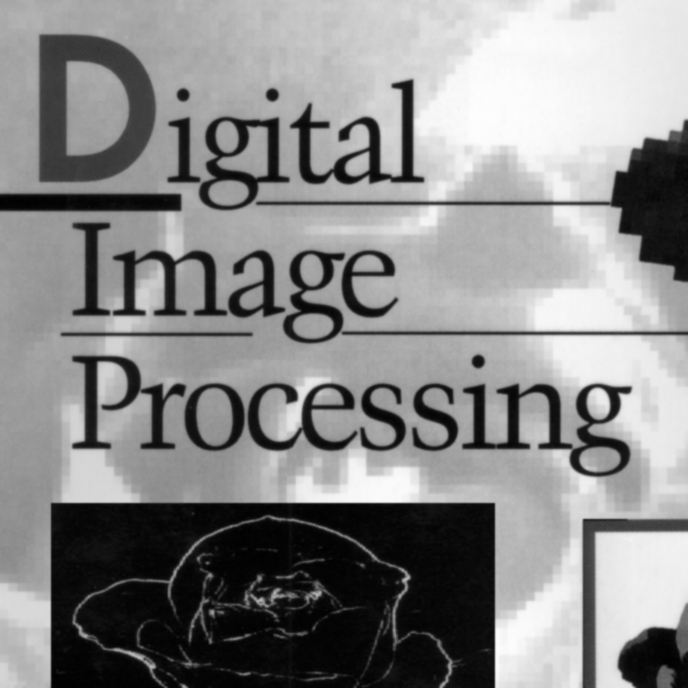
\includegraphics[width=1.0\textwidth]{tp.jpg} 
\end{figure}  
\end{textblock}
\end{center}

% \begin{textblock}{1}(.1,.21)
%     \noindent{\fontsize{30}{2}\selectfont
%         \bfseries\textcolor{white}{for \LaTeX}}
% \end{textblock}

\begin{comment}

\begin{textblock}{.9}(.05,.56)
    \begin{flushright}
        \noindent {\fontsize{20.74}{2}\selectfont
            \bfseries\textcolor{orange}{}}
    \end{flushright}
\end{textblock}


\begin{textblock}{.45}(.5,.82)
    \begin{center}
        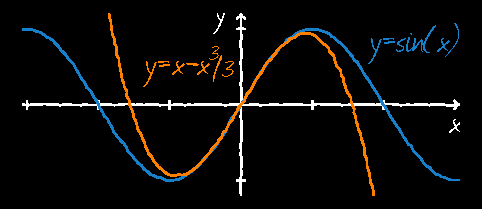
\includegraphics[width=.45\paperwidth]{dlsin}
    \end{center}
\end{textblock}

\begin{textblock}{.4}(.05,.65)
    \begin{center}
        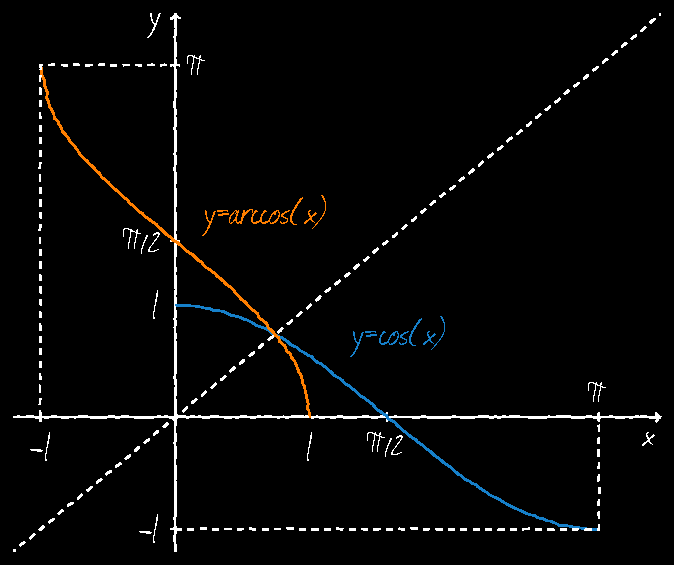
\includegraphics[width=.4\paperwidth]{arccos}
    \end{center}
\end{textblock}

\begin{textblock}{.6}(.05,.6)
    \noindent {\fontsize{20.74}{18}%
    \textcolor{white}{$\displaystyle(a+b)^n = \sum_{k=0}^n 
                \binom{n}{k} a^kb^{n-k}$}}
\end{textblock}


\begin{textblock}{.4}(.4,.77)
    \noindent {\fontsize{17.28}{18}%
    \textcolor{white!80}{$\displaystyle 
                \neg (p\vee q) \equiv (\neg p)\wedge (\neg q)$}}
\end{textblock}

\begin{textblock}{.4}(.1,.93)
    \noindent {\fontsize{14.4}{18}%
    \textcolor{white!50}{$\displaystyle 
                \binom{n}{k} = \frac{n!}{k!(n-k)!}$}}
\end{textblock}


\begin{textblock}{.6}(.5,.69)
    \noindent {\fontsize{17.28}{18}%
    \textcolor{white!10}{$\displaystyle 
                \zeta_k = |a|^{1/n} \mathrm{e}^{i(\mathrm{arg}(a)+2k\pi)/n}$}}
\end{textblock}


\begin{textblock}{.3}(.75,.73)
    \noindent {\fontsize{17.28}{18}%
    \textcolor{white!10}{$\displaystyle \mathrm{e}^{i\pi}+1=0$}}
\end{textblock}
\end{comment}


\null\newpage\pagestyle{nexus}